\documentclass{article}
\usepackage{graphicx}

\date{\today}
\author{Tarik Atlaoui \\ Nicolas Peugnet \\ Kimmeng Ly \\ Max Eliet}

\begin{document}


\begin{titlepage}
	\enlargethispage{2cm}
	\newcommand{\HRule}{\rule{\linewidth}{0.5mm}}
	\center
	\textsc{\LARGE
	Pre-rapport du PSAR 
	} \\[1cm]
	\HRule \\[0.4cm]
	{ \huge \bfseries API générique pour le développement d'applications réparties \\[0.15cm] }
	\HRule \\[4cm]
	\large{Tarik Atlaoui \\[3mm] Nicolas Peugnet \\[3mm] Kimmeng Ly \\[3mm] Max Eliet} \\[3cm]
	09 Mars 2020 \\[3cm]
%	\hfill 
\includegraphics[width=5cm]{logoSU.jpg}
\end{titlepage}

	\newpage
	\pagenumbering{arabic}
		\section{Introduction}
			\large{
			\indent Notre projet a pour but d'implémenter un intergiciel permettant l'execution d'applications réparties, aussi bien sur une infrastructure réelle que sur un simulateur, sans avoir à en modifier le code, afin de simplifier le développement de futures applications réparties.
\\[2mm]
			 \indent Dans notre cas, nous avons choisi d'implémenter cet intergiciel pour MPI (Message Passing Interface) en tant qu'API d'infrastructure réelle, et PeerSim en tant que simulateur à événements discrets.}
		
		\section{Les mots clés retenus}
		-PeerSim
		\newline
		-MPI
		\newline
		-Message Passing Interface
		\newline
		-Distributed systems
		\newline
		-p2p simulator
		\newline
		-Simulation of Distributed systems
		\newline
		-distributed algorithms
		\newline
		-Naimi and Trehel algorithm
		\newline
		-Ring algorithm
		\newline 
		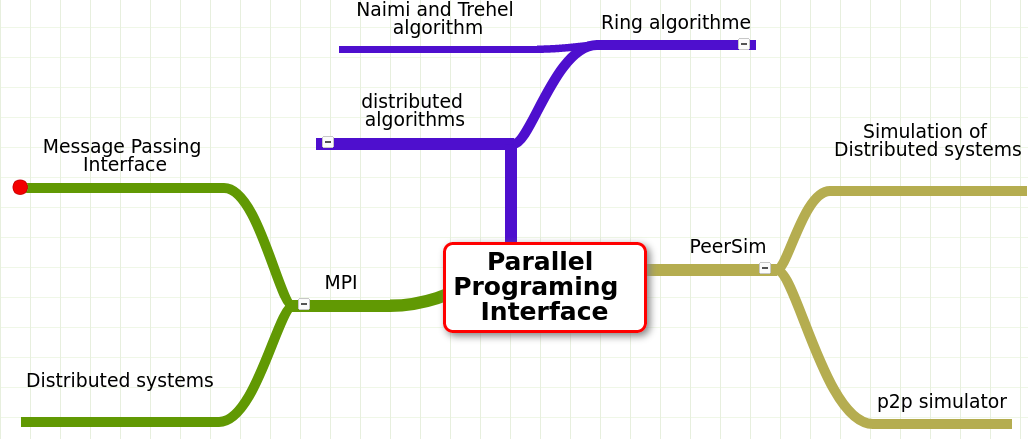
\includegraphics[width=10cm]{mindmap.png}
		\section{Descriptif de la recherche documentaire}
		\indent Nous avons commencé par comprendre ce qu'est un systeme distribué et comment fonctionnent les systemes MPI et PeerSim à travers quelques exemples d'algorithmes que nous avons implémenté dans chaqu'
		\indent une des API ,nous avons aussi utilisé google scholar pour comprendre comment la communauté utilise les deux API et pour avoir la version exacte et prouver des algorithmes que nous avons utilisé
		\indent car pour les algorithmes il est facile de passer à côté et beaucoup de gens implémentent des versions fonctionnelles mais qui n'appliquent pas vraiment l'algorithme c'est pour ça que nous avons utilisé
		\indent la description de l'algorithme sortie direct des thèses des inventeurs , pour les deux API nous avons utilisé les manuels des developpeurs qui ont crée les deux applications pour mieux comprendre 
		\indent les subtilités de celles-ci nous avons utilisé la documentation des inventeurs car elle est précise et bien détaillée.
		\newline
		\indent Nous avons beaucoup utilisé google scholar car il a une quantité impressionante de ressources et qu'elles sont pour la plupart des sources fiables et cela nous a permis d'acceder aux thèses qui nous
		\indent intéressaient, aussi nous avons utilisé la doc du langage Java , puisque ça a été le langage d'implantation de notre interface.

		
		\section{Bibliographie produite dans le cadre du projet}

		\section{Evaluation des sources}

\end{document}